\section{Исследовательский раздел}

\subsection{Технические характеристики}

Технические характеристики устройства, на котором выполнялись замеры, следующие.

\begin{itemize}[label=---]
	\item Операционная система Windows 10 \cite{oswind} x86\_64.
	\item Память 8 Гб 2400 МГц DDR4.
	\item 1.6 ГГц 4-ядерный процессор Intel Core i5 8265U \cite{intel}.
\end{itemize}

Замеры проводились на ноутбуке, включенном в сеть электропитания. Во время проведения исследований ноутбук был нагружен только встроенными приложениями окружения, а также непосредственно системой выполнения замеров.

\subsection{Подготовка исследования}

Для выявления зависимости времени исполнения запросов от использования кеширующей СУБД база данных была пополнена текстами на французском и немецком языках.
База данных заполнена более чем тридцатью предложениями и более чем 500 словами. 
На момент начала замеров кеширующая СУБД пуста.

Замеры производятся для двух запросов на получение примеров употребления слова в корпусе.
\begin{enumerate}
	\item Поиск перевода французского слова <<nous>> (рус. <<мы>>) на немецкий язык: api/v1/corpus/\{uuid\}/concordance?Word=nous\&LanguageCode=de. 
	Далее \\обозначим этот запрос как <<простой>>, поскольку он не предполагает фильтрацию.
	
	\item  Поиск перевода французского слова <<nous>> на немецкий язык среди текстов <<Описательного>> жанра, написанные с 1 января 2000 по 14 мая 2023: api/v1/corpus/\{uuid пользователя\}/concordance?Word=nous\&LanguageCo-de=de\&Filter.Genre=Description\&Filter.StartDateTime=01.01.2000\&Filter.\\EndDateTime=05.14.2023. 
	Обозначим этот запрос как <<сложный>>, поскольку он потребует больше соединений таблиц.
\end{enumerate}

\subsection{Результаты замеров}
На рисунке \ref{cache-comparison} представлено время выполнения <<простого>> запроса методом GetConcordance класса LanguageRepository, который выполняет проверку на наличие в кеше данных по запросу и непосредственное выполнение запросов к базе данных.

\captionsetup{singlelinecheck = false, justification=centering}
\begin{figure}[ht]
	\centering
	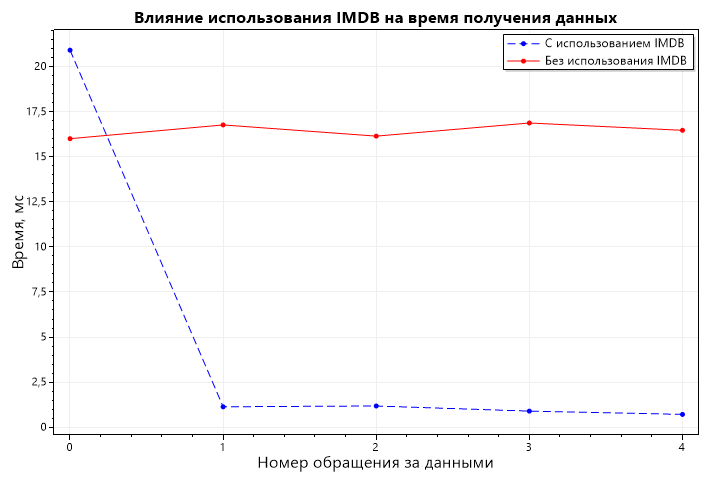
\includegraphics[scale=0.8]{img/plots/cache-comparison}
	\caption{Время выполнения <<простого>> запроса методом GetConcordance}
	\label{cache-comparison}
\end{figure}\clearpage

Как видно из полученных данных, после первого обращения за данными время их получения уменьшается более чем в 20 раз. Время выполнения <<простого>> запроса без использования кеширующей СУБД не зависит от номера обращения за данными.

Аналогичные результаты получены для <<сложного>> запроса. Время его выполнения представлено на рисунке \ref{cache-comparison-complex}.
\begin{figure}[ht]
	\centering
	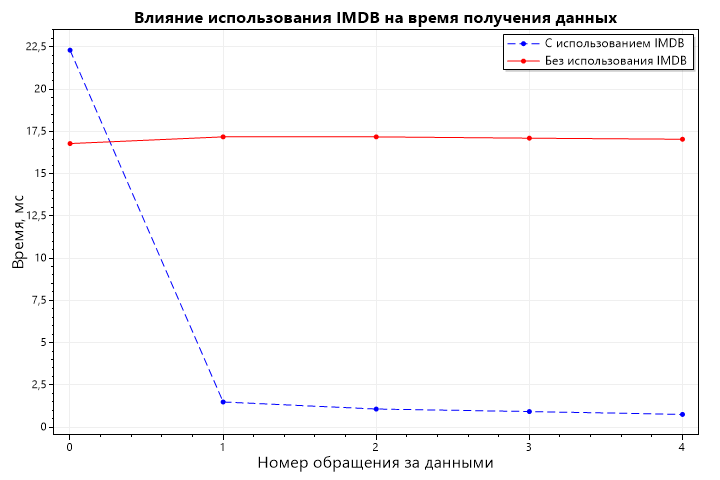
\includegraphics[scale=0.8]{img/plots/cache-comparison-complex}
	\caption{Время выполнения <<сложного>> запроса методом GetConcordance}
	\label{cache-comparison-complex}
\end{figure}

Данные, представленные на рисунках \ref{cache-comparison} и \ref{cache-comparison-complex}, получены вследствие усреднения результатов 500 замеров времени выполнения запросов с одними и теми же входными данными.

С помощью программы Apache JMeter~\cite{jmeter} было проведено нагрузочное тестирование системы. 
Результаты замеров времени ответа системы на <<простой>> запрос с использованием и без использования кеширующей СУБД представлены на рисунках \ref{http-with-cache} и \ref{http-no-cache} соответственно.

\begin{figure}[H]
	\centering
	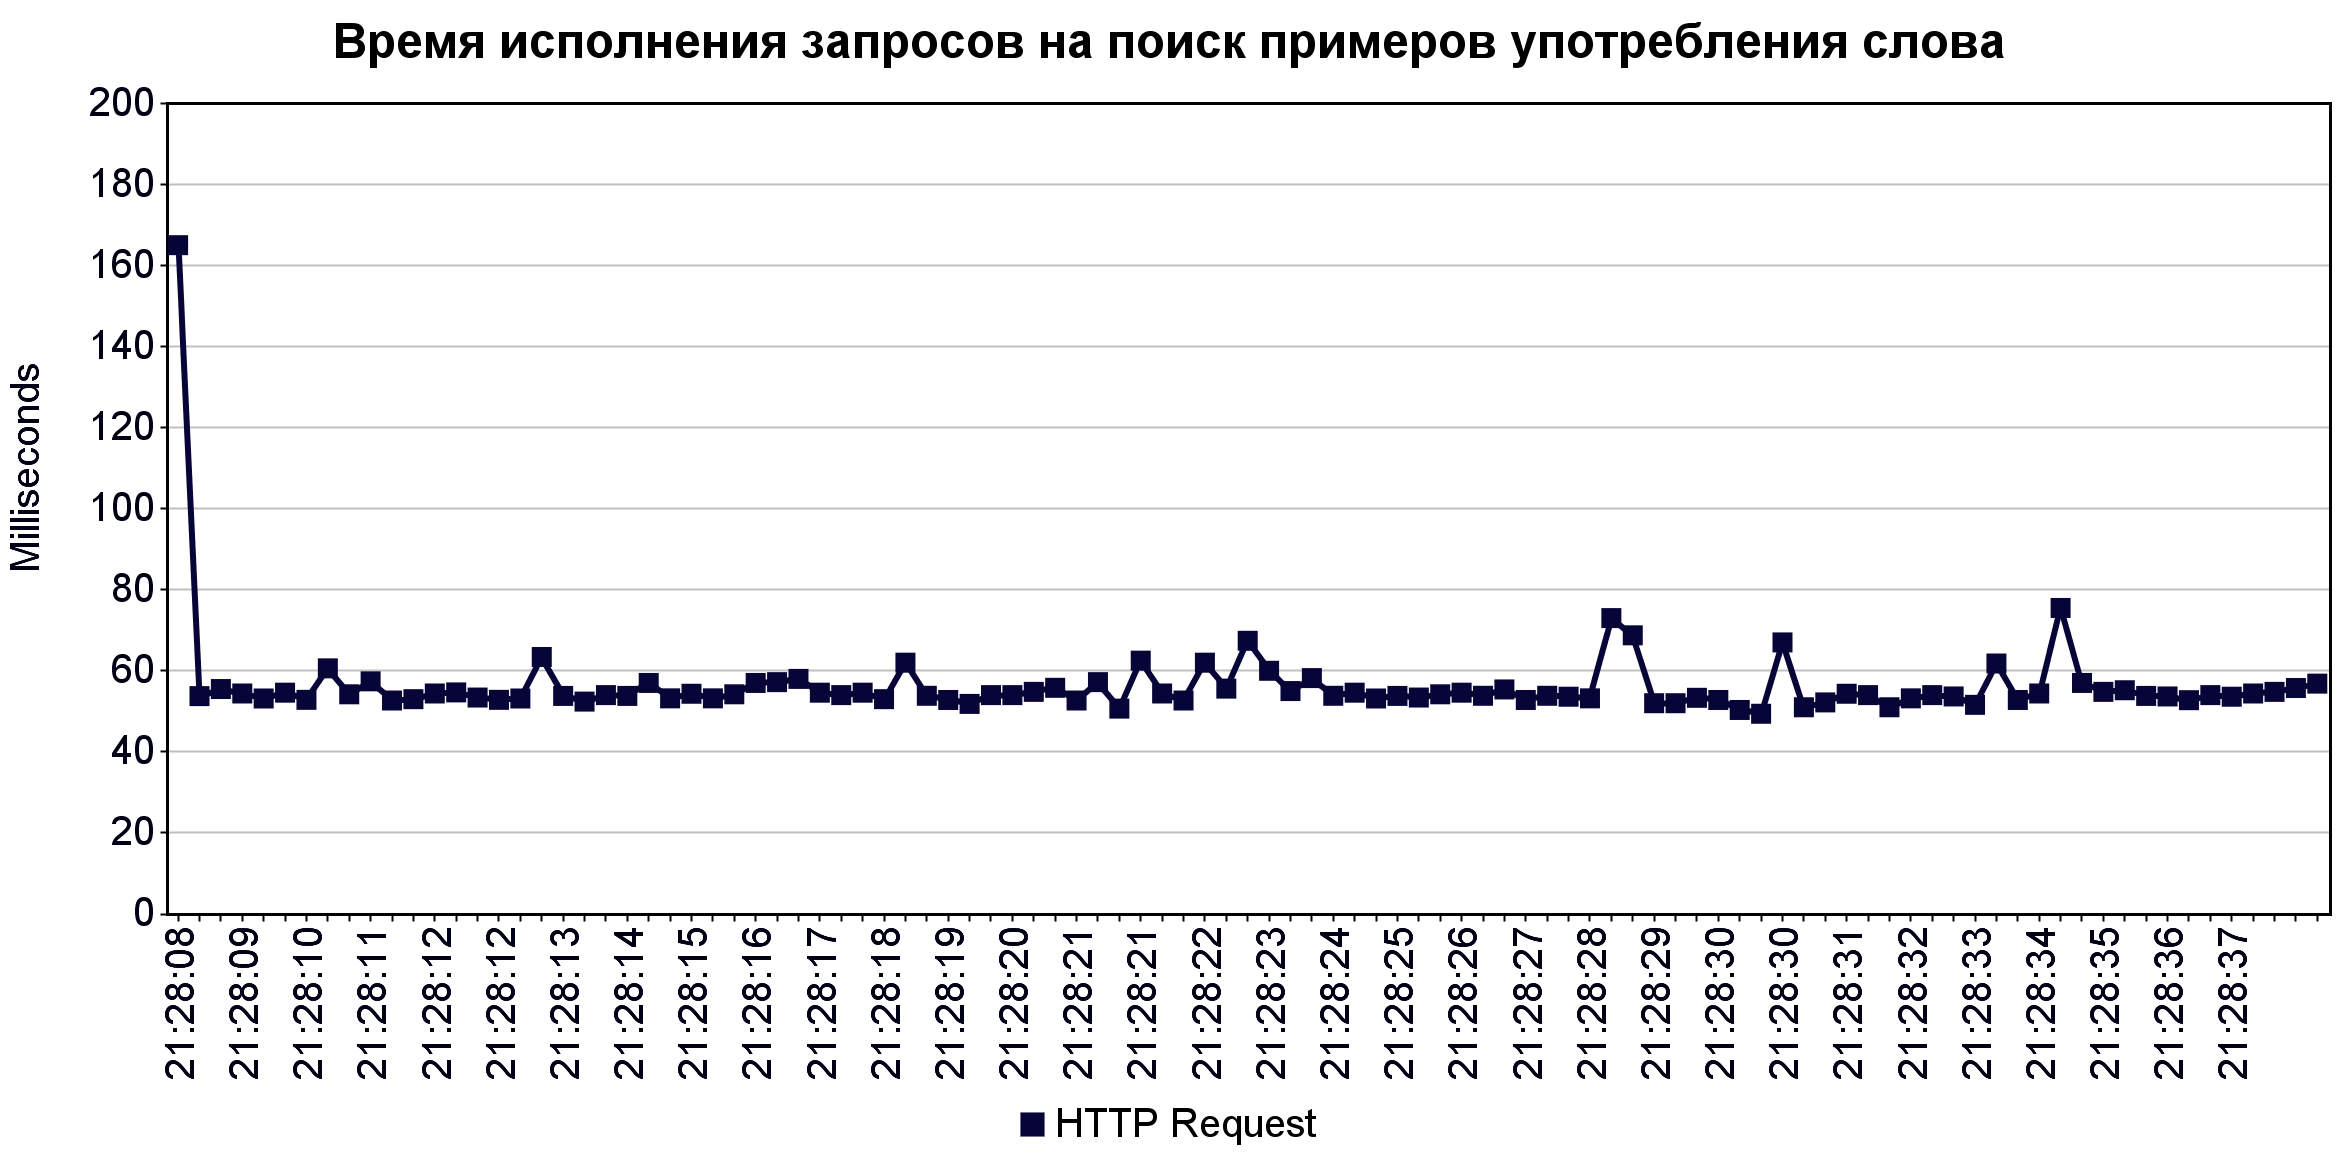
\includegraphics[width=\textwidth]{img/plots/http-with-cache}
	\caption{Время выполнения <<простого>> запроса к системе с использованием кеширующей СУБД}
	\label{http-with-cache}
\end{figure}

\begin{figure}[ht]
	\centering
	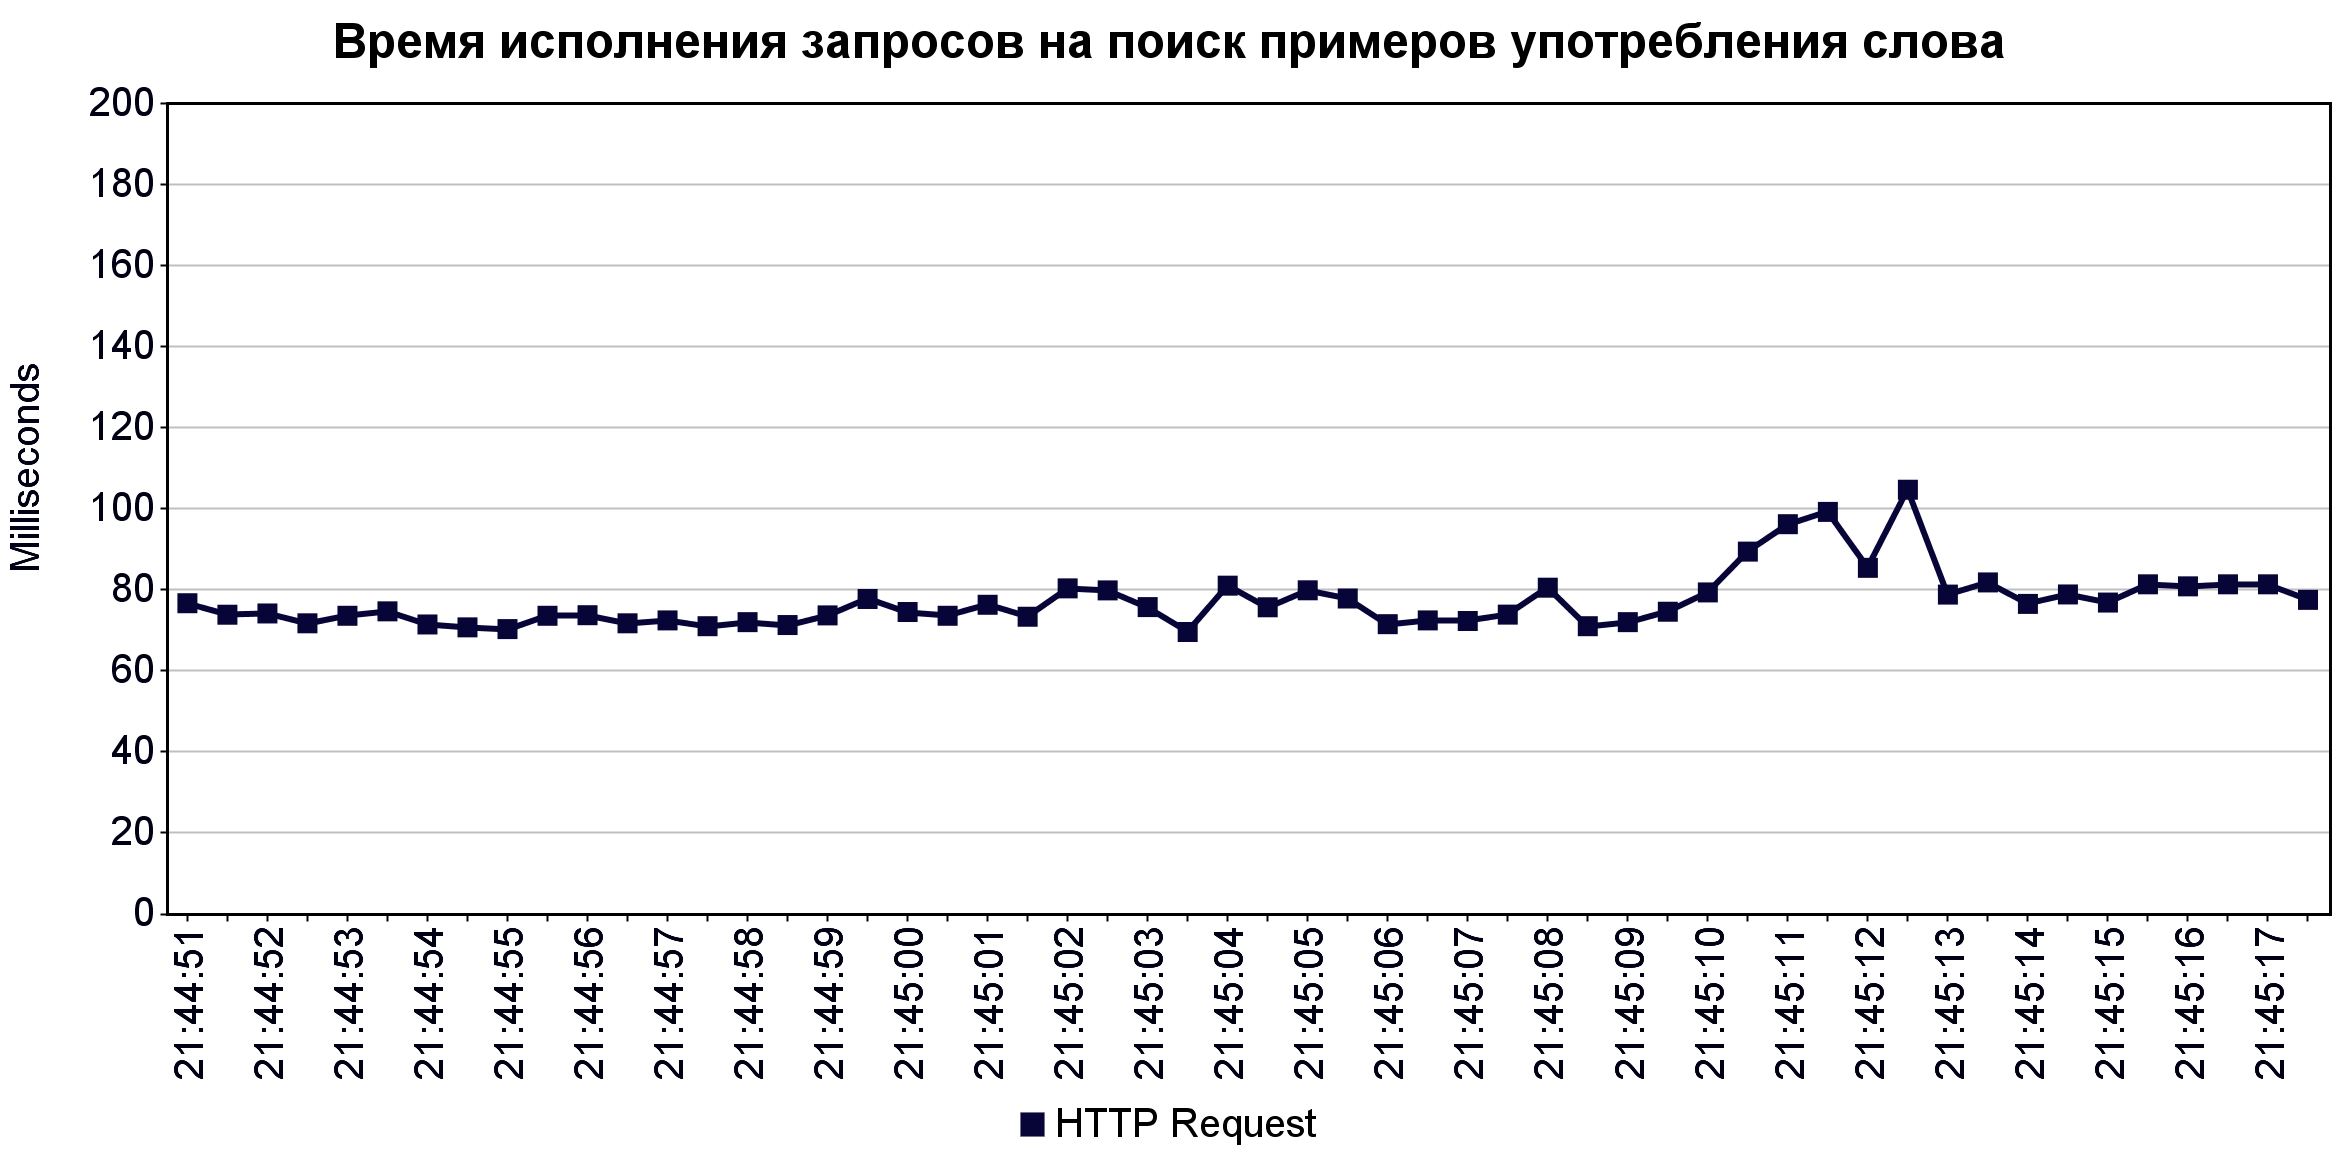
\includegraphics[width=\textwidth]{img/plots/http-no-cache}
	\caption{Время выполнения <<простого>> запроса к системе без использования кеширующей СУБД}
	\label{http-no-cache}
\end{figure}\clearpage

На рисунках \ref{http-complex-with-cache} и \ref{http-complex-no-cache} представлены аналогичные замеры для <<сложного>> запроса.

\begin{figure}[ht]
	\centering
	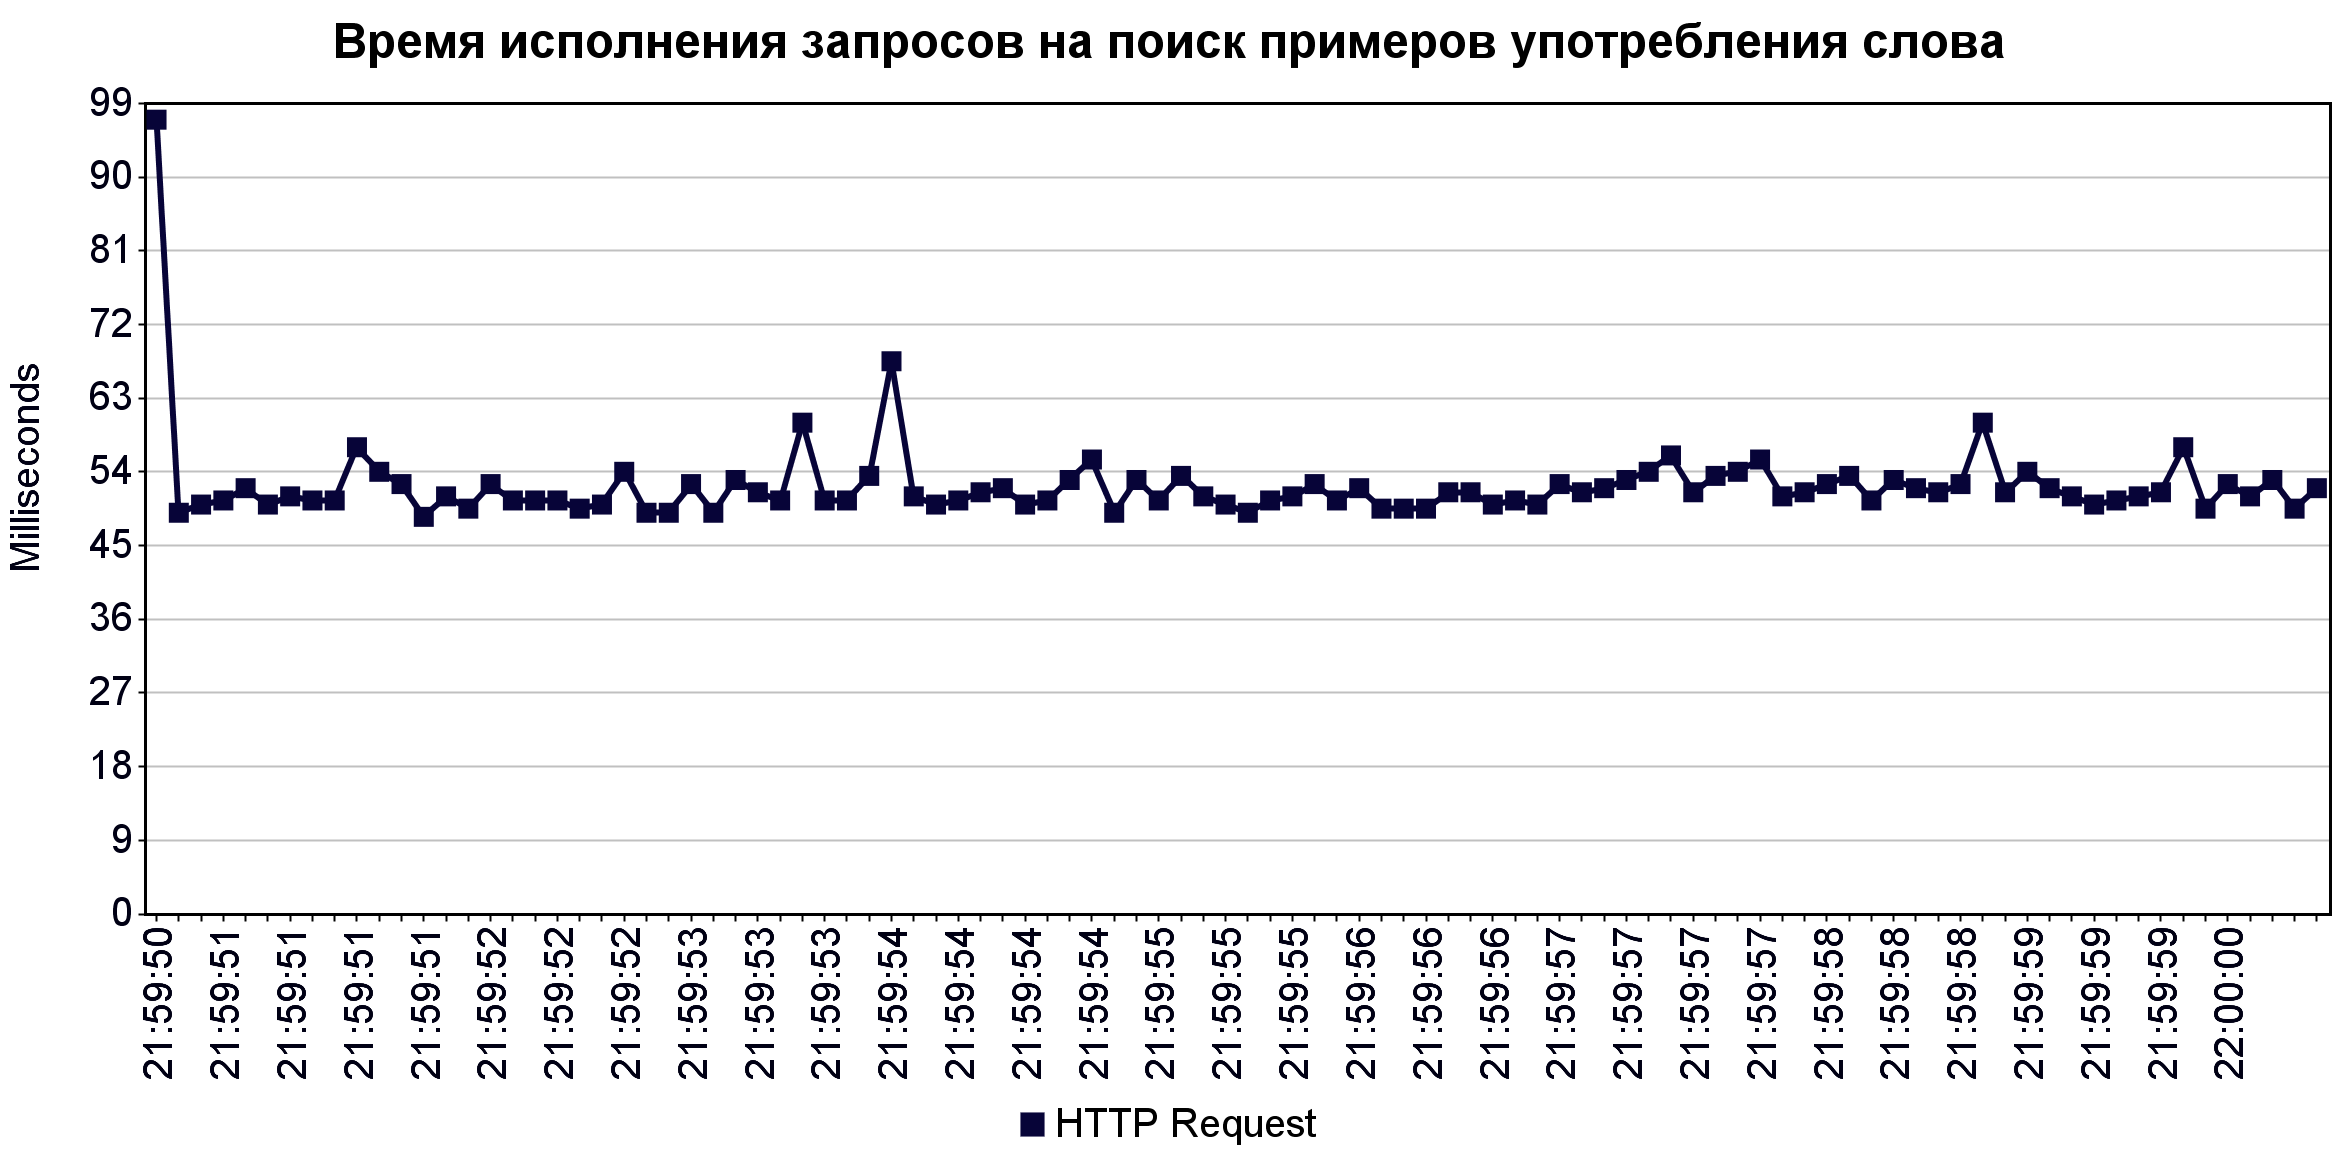
\includegraphics[scale=0.35]{img/plots/http-complex-with-cache}
	\caption{Время выполнения <<сложного>> запроса к системе с использованием кеширующей СУБД}
	\label{http-complex-with-cache}
\end{figure}

\begin{figure}[ht]
	\centering
	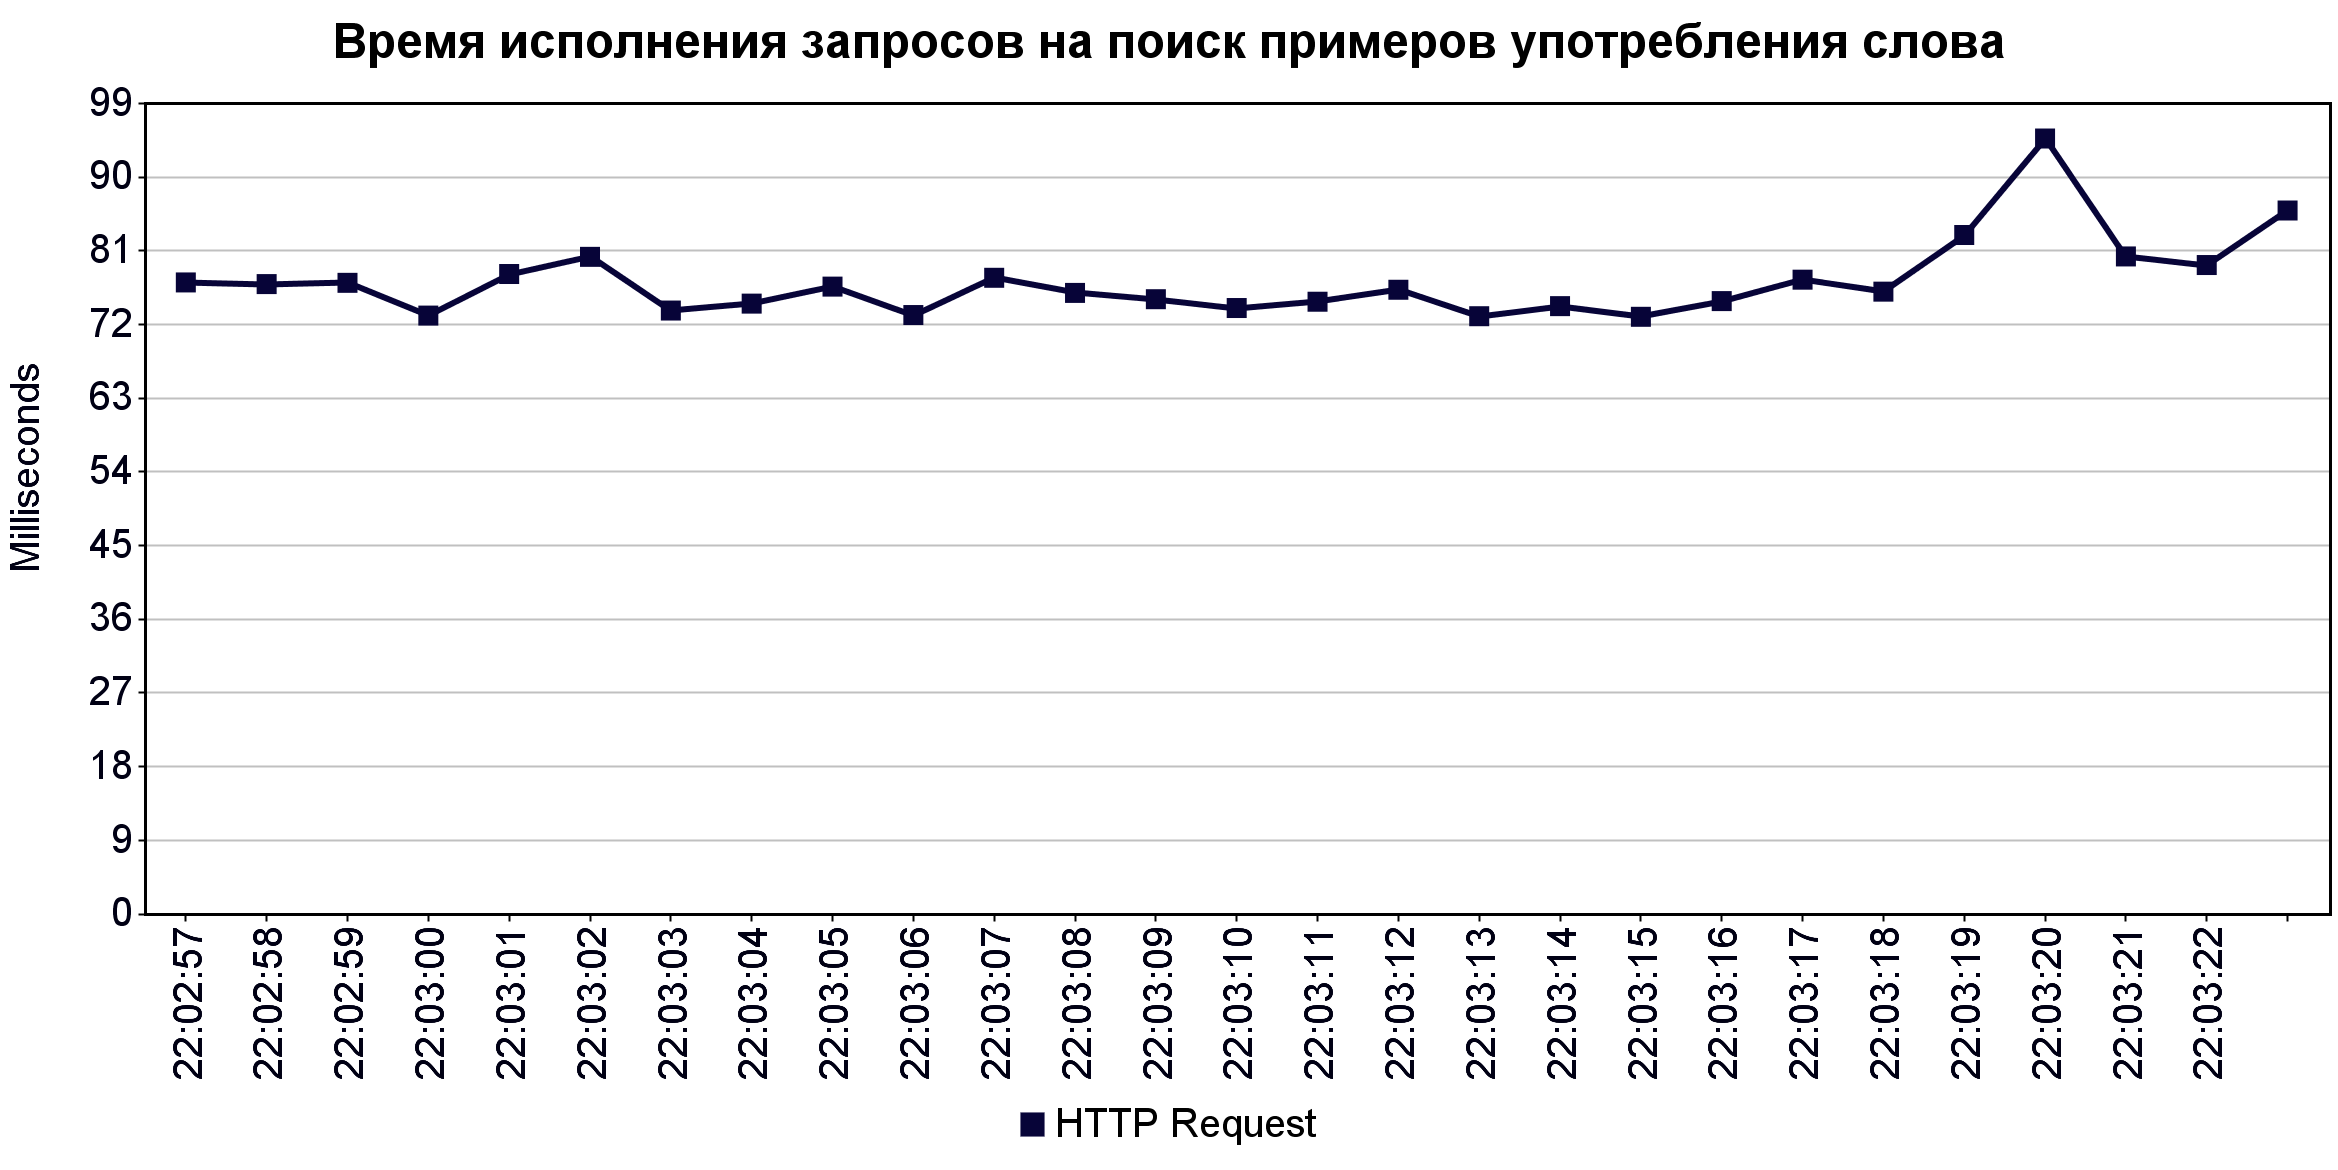
\includegraphics[scale=0.35]{img/plots/http-complex-no-cache}
	\caption{Время выполнения <<сложного>> запроса к системе без использования кеширующей СУБД}
	\label{http-complex-no-cache}
\end{figure}\clearpage

Таким образом, благодаря использованию кеширующей СУБД, время получения ответа как на <<простой>>, так и на <<сложный>> запрос уменьшается на 25\%: с 80 мс до 60 мс. 
Однако, в случае использования кеширующей СУБД, при первом получении запроса необходимо записать значение в кеш.

\subsection*{Вывод}

В результате проведенных замеров и, в том числе нагрузочного тестирования, установлено, что использование кеширующей СУБД позволяет сократить время повторного получения данных на 25\%. 
Однако, в связи с необходимостью записи данных в кеширующую СУБД, время получения ответа на новый запрос увеличивается.

\pagebreak